\documentclass{article}%
\usepackage[T1]{fontenc}%
\usepackage[utf8]{inputenc}%
\usepackage{lmodern}%
\usepackage{textcomp}%
\usepackage{lastpage}%
\usepackage{graphicx}%
%
\usepackage[utf8]{inputenc}%
\usepackage{graphicx}%
\usepackage{amsmath}%
\usepackage{caption}%
\usepackage{subcaption}%
\usepackage[margin=1in]{geometry}%
\title{Report : Max-Cut Problem Analysis}%
\author{Khalid Hasan Tuhin - 2105002}%
\date{\today}%
%
\begin{document}%
\normalsize%
\maketitle%
\section{High{-}Level Algorithm Descriptions}%
\label{sec:High{-}LevelAlgorithmDescriptions}%
The following algorithms were implemented to solve the Max{-}Cut problem:%
\begin{itemize}%
\item \textbf{Randomized}: Assigns vertices to partitions \(X\) or \(Y\) randomly with equal probability, averaging results over multiple iterations.%
\item \textbf{Greedy}: Starts with the edge of maximum weight, greedily assigning remaining vertices to maximize the current cut.%
\item \textbf{Semi-Greedy}: Uses a restricted candidate list based on a greedy function and random selection, balancing greediness and randomness.%
\item \textbf{Local Search}: Improves an initial solution by iteratively moving vertices to the partition that maximizes the cut until no further improvement is possible.%
\item \textbf{GRASP}: Combines semi-greedy construction with local search, iterating multiple times to find the best solution.%
\end{itemize}

%
\section{Comparison of Algorithms}%
\label{sec:ComparisonofAlgorithms}%
Based on the results, the performance of algorithms varies across graphs:%
\begin{itemize}%
\item For graph G1:%
\begin{itemize}%
\item Randomized: 9585%
\item Greedy: 10956%
\item Semi-Greedy: 11203%
\item Local Search: 11366 (after 5 iterations)%
\item GRASP: 11432 (after 5 iterations)%
\item Known Best: 12078%
\end{itemize}%
\item For graph G2:%
\begin{itemize}%
\item Randomized: 9596%
\item Greedy: 11030%
\item Semi-Greedy: 11116%
\item Local Search: 11389 (after 5 iterations)%
\item GRASP: 11408 (after 5 iterations)%
\item Known Best: 12084%
\end{itemize}%
\item For graph G3:%
\begin{itemize}%
\item Randomized: 9586%
\item Greedy: 11012%
\item Semi-Greedy: 11172%
\item Local Search: 11350 (after 5 iterations)%
\item GRASP: 11409 (after 5 iterations)%
\item Known Best: 12077%
\end{itemize}%
\item For graph G4:%
\begin{itemize}%
\item Randomized: 9583%
\item Greedy: 11031%
\item Semi-Greedy: 11230%
\item Local Search: 11382 (after 5 iterations)%
\item GRASP: 11441 (after 5 iterations)%
\item Known Best: N/A%
\end{itemize}%
\item For graph G5:%
\begin{itemize}%
\item Randomized: 9588%
\item Greedy: 10990%
\item Semi-Greedy: 11235%
\item Local Search: 11380 (after 5 iterations)%
\item GRASP: 11446 (after 5 iterations)%
\item Known Best: N/A%
\end{itemize}%
\item For graph G6:%
\begin{itemize}%
\item Randomized: 75%
\item Greedy: 1515%
\item Semi-Greedy: 1624%
\item Local Search: 1915 (after 5 iterations)%
\item GRASP: 1960 (after 5 iterations)%
\item Known Best: N/A%
\end{itemize}%
\item For graph G7:%
\begin{itemize}%
\item Randomized: -82%
\item Greedy: 1362%
\item Semi-Greedy: 1524%
\item Local Search: 1779 (after 5 iterations)%
\item GRASP: 1829 (after 5 iterations)%
\item Known Best: N/A%
\end{itemize}%
\item For graph G8:%
\begin{itemize}%
\item Randomized: -84%
\item Greedy: 1331%
\item Semi-Greedy: 1478%
\item Local Search: 1776 (after 5 iterations)%
\item GRASP: 1830 (after 5 iterations)%
\item Known Best: N/A%
\end{itemize}%
\item For graph G9:%
\begin{itemize}%
\item Randomized: -27%
\item Greedy: 1507%
\item Semi-Greedy: 1557%
\item Local Search: 1779 (after 5 iterations)%
\item GRASP: 1804 (after 5 iterations)%
\item Known Best: N/A%
\end{itemize}%
\item For graph G10:%
\begin{itemize}%
\item Randomized: -78%
\item Greedy: 1350%
\item Semi-Greedy: 1531%
\item Local Search: 1745 (after 5 iterations)%
\item GRASP: 1783 (after 5 iterations)%
\item Known Best: N/A%
\end{itemize}%
\end{itemize}%
GRASP tends to perform closest to the known best solutions across graphs, indicating its effectiveness. Local Search values are notably lower, suggesting potential issues with local optima or initial partitions. Randomized consistently underperforms due to its lack of optimization.

%
\section{Visualization}%
\label{sec:Visualization}%


\begin{figure}[h!]%
\centering%
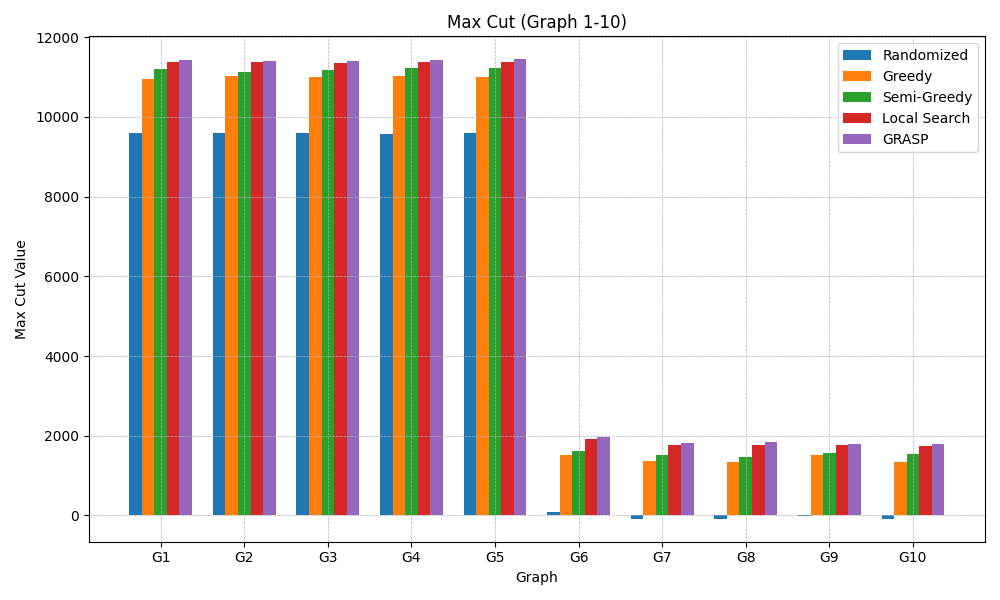
\includegraphics[width=0.8\textwidth]{max_cut_plot.png}%
\caption{Max Cut Values for Graphs G1{-}G10}%
\end{figure}

%
\end{document}